\section{Optimization model and solution strategy}\label{sec:OptimizationModel}

In this section, the optimization problem is presented. First, the time sequence of decisions for participation in mFRR is presented. Second, we explain how scenarios for price data are generated for learning a good policy in-sample (IS). Here, two strategies are introduced: 1) A simple one looking only at 2021 price data and 2) A dynamic one looking at the past five days of spot prices. Third, we present the compact model formulation. Fourth, we present how the mFRR bidding policy is implemented. Lastly, we show how scenario decomposition with ADMM is used to solve the first strategy with up to 250 scenarios.

\subsection{Time sequence for decision making}

Figure \ref{fig:timeline_mfrr_variables} shows the stages for making decisions in the mFRR market. First, a reservation bid $p_{h}^{r,\uparrow}$ is submitted. For any reservation bid accepted, a regulating power bid must be submitted, $\lambda_{h,\omega}^{\text{bid}}$. The reservation and bid are the \textit{first-stage} decisions. The set $\Gamma_{\omega}$ contains all real-time variables in the optimization problem and are the \textit{second-stage} decisions. They control the real-time power, auxiliary variables for identifying up- and down-regulation\footnote{Down-regulation refers to the rebound action in this context.}, temperature dynamics, and when to deliver up-regulation according to the bid and prices (see Appendix A for a detailed description). Index $\omega$ specifies a scenario.
% \begin{figure}[!t]\label{fig:timeline_mfrr_variables}
%     \centering
%     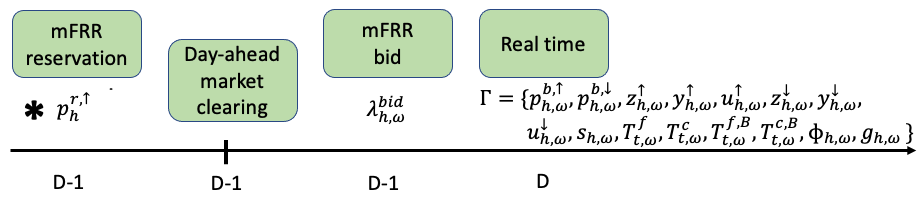
\includegraphics[width=\columnwidth]{../figures/timeline_mfrr_variables.png}
%     \caption{Variables related to mFRR up-regulation decisions. The asterisk indicates the first-stage decision.}
% \end{figure}

\begin{figure}[!t]
    \centering
    \includestandalone[width=\columnwidth]{../figures/timeline_mfrr_variables_tikz}
    \caption{Variables related to mFRR up-regulation decisions. The asterisk indicates the first-stage decision, and \\ $\Gamma_{\omega} = \{ \bm{p}^{r,\uparrow}, \bm{\lambda}_{\omega}^{\text{bid}}, \bm{p}_{\omega}^{b,\uparrow}, \bm{p}_{\omega}^{b,\downarrow}, \bm{s}_{\omega}, \bm{T}_{\omega}^{c}, \bm{T}_{\omega}^{f}, \bm{T}_{\omega}^{c, B}, \bm{T}_{\omega}^{f,B}, \bm{\phi}_{\omega}, \bm{g}_{\omega} \}$ is the set of second-stage decision variables.}
    \label{fig:timeline_mfrr_variables}
\end{figure}

\subsection{Scenario generation}\label{sec:scenario_generation}

To learn a good policy for reservation capacity and bidding, i.e., $p_{h}^{r,\uparrow}$ and $\lambda_{h,\omega}^{\text{bid}}$, we generate scenarios for price data using two different strategies (where one scenario corresponds to one day):

\begin{enumerate}
    \item Policy learned on 2021 price data with $\omega \in \Omega = \{ 1, 5, 10, 20, 30, 40, 50, 100, 250 \}$ scenarios.
    \item Policy learned using a lookback of five days for spot prices.
\end{enumerate}

In both cases, balancing prices, $\lambda_{h,\omega}^{b}$, are sampled in the following way. First, an integer $x$ is sampled uniformly from $\{0 \ldots 24\}$ which represents the total number of up-regulation hours in a day. We then sample price differentials ($\bm{\lambda}^{b}-\bm{\lambda}^{s}$) from a single day from the set of all days where up-regulation happened $x$ times. This constitutes one scenario and is repeated $|\Omega|$ times. In this way, days where up-regulation happened are essentially up-sampled, and the model learns more when up-regulation happens than otherwise.

For spot prices, the lookback strategy uses the spot prices from the past five days to take advantage of any autocorrelation, whereas the first strategy samples spot prices from 2021. For both strategies, evaluation is done out-of-sample (OOS) on unseen 2022 price data.

For load shifting, the policy is simply to solve the optimization problem for the next day since the day-ahead market clearing happens in advance.

\subsection{Compact model formulation}

The compact model formulation is presented in Problem (\ref{P1:compact_model}). The objective function is the sum of the revenue from the reservation bid, i.e., first-stage decisions, and the \textit{expected} revenue and costs from the regulating power bid and subsequent rebound and penalties. Constraint (\ref{P1:eq2}) incorporates activation of the bid, and constraint (\ref{P1:eq3}) incorporates the temperature dynamics in the freezer.


\begin{subequations}\label{P1:compact_model}
    \begin{align}
        \underset{\bm{p}^{r,\uparrow}, \bm{\lambda}_{\omega}^{\text{bid}}, \bm{\Gamma}_{\omega}}{\textrm{max}} \quad & f(\bm{p}^{r,\uparrow}) + \sum_{\omega \in \Omega} \pi_{\omega} g(\bm{\Gamma}_{\omega}) \label{P1:eq1}
        \\
        s.t \quad                                                                                                    & h(\bm{p}^{r,\uparrow}, \bm{\lambda}_{\omega}^{\text{bid}}, \bm{\Gamma}_{\omega}) \leq 0, \quad \forall{\omega}\label{P1:eq2}                                                                     \\
        \quad                                                                                                        & \text{State-space model in } (\ref{eq:2ndFreezerStateSpace}), \quad \forall{\omega} \label{P1:eq3}
        \\
        \quad                                                                                                        & \Bigl( \bm{p}^{r,\uparrow}, \bm{\lambda}_{\omega}^{\text{bid}}, \bm{p}_{\omega}^{b,\uparrow}, \bm{p}_{\omega}^{b,\downarrow}, \bm{s}_{\omega}, \bm{T}_{\omega}^{c}, \bm{T}_{\omega}^{f}, \notag \\ \quad & \quad \bm{T}_{\omega}^{c, B}, \bm{T}_{\omega}^{f,B}, \bm{\phi}_{\omega}, \bm{g}_{\omega} \Bigr) \in \mathbb{R}^{n}  \label{P1:eq4}
        \\
        \quad                                                                                                        & \bm{u}_{\omega}, \bm{z}_{\omega}, \bm{y}_{\omega} \in \{0,1\}  \label{P1:eq5}
    \end{align}
\end{subequations}

For mFRR, the objective function in (\ref{eq:mFRRObjective}) corresponds to $f$ and $g$ in (\ref{P1:eq1}). For load shifting, the optimization problem is simply obtained by removing bid constraints and replacing the (\ref{P1:eq1}) with (\ref{eq:LoadShiftingObjective}), and then solving the optimization problem for the next day.


\subsection{mFRR bidding implementation}\label{sec:mFRR_bidding_implementation}

To solve Problem (\ref{P1:compact_model}), we first need to specify a bidding policy that can readily be used OOS. We do so by choosing an affine bidding policy. Afterwards, it is shown how the bidding policy is implemented using McCormick relaxation.

\subsubsection{Affine bidding policy}

A bidding policy needs to be easy to follow OOS for the trader. We choose an affine bidding policy, i.e., a linear function of the spot price. The bidding policy is given by:

\begin{subequations}\label{eq:affine_policy}
    \begin{align}
        \lambda^{bid}_{h,\omega}           & = \label{affine_policy:1} \\  
        & \alpha ( \underbrace{\lambda_{h+1,\omega}^{s} - \lambda_{h,\omega}^{s}}_{\lambda_{h,\omega}^{s,\text{diff}}} ) + \beta + \lambda_{h,\omega}^{s}, \quad \forall{\omega}, \forall{h} \in \{1\ldots23\} \nonumber \\
        \alpha                             & \geq 0\label{affine_policy:2}                                                                                                                            \\
        \beta                              & \geq 0\label{affine_policy:3}
    \end{align}
\end{subequations}

The idea in (\ref{eq:affine_policy}) is that the spot price difference approximates a reasonable policy since a large price differential in hour $h$ means that the spot price at time $h+1$ is much higher. Hence, a large bid at time $h$ is desirable such that the probability of being activated in hour $h$ and rebounding in an expensive hour $h+1$ is low (cf. Section \ref{sec:mFRR}).

Variables $\alpha$ and $\beta$ are then learned IS and fixed for OOS evaluation. After the day-ahead market clearing, (\ref{eq:affine_policy}) can easily be used to specify bids for the next day.

\subsubsection{McCormick relaxation}\label{sec:mccormick}

As explained in Section \ref{sec:mFRR}, activation of mFRR reservation only happens when certain price conditions are met. This is formalized in the following constraint:

\begin{equation}\label{eq:bid_constraint}
    p^{b, \uparrow}_{h,\omega} + s_{h,\omega} \geq p^{r,\uparrow}_{h} \cdot \mathbbm{1}_{h,\omega}^{(\lambda^{bid}_{h} < \lambda^{b}_{h,\omega} \land \lambda^{b}_{h,\omega} > \lambda^{s}_{h})}, \quad \forall{h,\omega}
\end{equation}

Eq. (\ref{eq:bid_constraint}) shows how real-time up-regulation plus a slack variable must be greater than or equal to the reservation if the bid is lower than the balancing price and if up-regulation is needed in hour $h$. It is a bi-linear constraint so McCormick relaxation \cite{mccormick1976computability} is used to convert (\ref{eq:bid_constraint}) to a linear constraint by introducing auxiliary variables, $\phi_{h,\omega}$ and $g_{h,\omega}$:

\begin{subequations}\label{eq:bid_constraint_relaxed}
    \begin{align}
        \lambda_{h,\omega}^{b} - \lambda_{h}^{s} \geq \lambda_{h,\omega}^{bid} - M \cdot (1 - g_{h,\omega}) , \quad                                   & \forall{h,\omega}             \label{con_bid:subeq1} \\
        \lambda_{h,\omega}^{bid} \geq \lambda_{h,\omega}^{b} - \lambda_{h}^{s} - M \cdot (1 - g_{h,\omega}) , \quad                                   & \forall{h,\omega}             \label{con_bid:subeq2} \\
        p^{b, \uparrow}_{h,\omega} \leq \phi_{h,\omega} \cdot \mathbbm{1}_{h,\omega}^{\lambda^{b}_{h,\omega} > \lambda^{s}_{h}}, \quad                & \forall{{h,\omega}}           \label{con_bid:subeq3} \\
        p^{b, \uparrow}_{h,\omega} + s_{h,\omega} \geq \phi_{h,\omega} \cdot \mathbbm{1}_{h,\omega}^{\lambda^{b}_{h,\omega} > \lambda^{s}_{h}}, \quad & \forall{{h,\omega}}           \label{con_bid:subeq4} \\
        -g_{h,\omega} \cdot M \leq \phi_{h,\omega}, \quad                                                                                             & \forall{h,\omega}             \label{con_bid:subeq5} \\
        \phi_{h,\omega} \leq g_{h,\omega} \cdot M, \quad                                                                                              & \forall{h,\omega}             \label{con_bid:subeq6} \\
        -(1 - g_{h,\omega}) \cdot M \leq \phi_{h,\omega} - p^{r,\uparrow}_{h}, \quad                                                                  & \forall{h,\omega}             \label{con_bid:subeq7} \\
        \phi_{h,\omega} - p^{r,\uparrow}_{h} \leq (1 - g_{h,\omega}) \cdot M, \quad                                                                   & \forall{h,\omega}             \label{con_bid:subeq8}
        % \lambda_{h,\omega}^{bid} \leq \lambda^{Max} \label{con_bid:subeq9}
    \end{align}
\end{subequations}

Constraints (\ref{con_bid:subeq1}-\ref{con_bid:subeq2}) ensures that $g_{h,\omega} = 1$ when the balancing price minus the spot price is larger than our bid, $\lambda^{bid}_{h, \omega}$, and zero otherwise. Constraints (\ref{con_bid:subeq3}-\ref{con_bid:subeq4}) sets the TCL up-regulation equal to $\phi_{h,\omega}$ (or incurs a penalty through $s_{h,\omega}$) if there is an up-regulation event in the system, i.e., if $\mathbbm{1}_{h,\omega}^{\lambda^{b}_{h,\omega} > \lambda^{s}_{h}} = 1$. Constraints (\ref{con_bid:subeq5}-\ref{con_bid:subeq6}) ensures that $\phi_{h,\omega} = 0$ when $g_{h,\omega} = 0$, i.e., when the balancing price differential is smaller than our bid. Constraints (\ref{con_bid:subeq7}-\ref{con_bid:subeq8}) ensures that $\phi_{h,\omega}$ is equal to the reservation capacity, $p^{r,\uparrow}_{h}$, whenever $g_{h,\omega} = 1$, i.e., whenever the bid is smaller than the balancing price differential.

The final model formulation is shown in its entirety in Appendix A.

\subsection{Scenario decomposition with ADMM}

When solving Problem (\ref{P1:compact_model}) using the first strategy with many scenarios, it quickly becomes computationally intractable due to the number of binaries and intertemporal constraints. To solve it, the ADMM algorithm is used which can solve a large-scale optimization problem by decomposing it into smaller subproblems \cite{boyd2011distributed}. In (\ref{P1:compact_model}), each scenario is solved as a subproblem by setting:

\begin{equation}\label{eq:non_anticipativity}
    \bm{p}^{r,\uparrow} \rightarrow \bm{p}^{r,\uparrow}_{\omega}, \quad \alpha \rightarrow \alpha_{\omega}, \quad \beta \rightarrow \beta_{\omega}
\end{equation}

The ADMM algorithm will converge by achieving consensus on first- and second-stage stage decisions in linear problems, but it is only a heuristic for MILPs \cite{hong2016convergence}.